\scanpage{4}
\deleted{par suite le deuxième membre de (8.1.4) est canoniquement dual à $\operatorname{Tors}^{n-1}(Y)\otimes_W k$. De même le premier membre est canoniquement \deleted{isomorphe à}\inserted{dual de} $\operatorname{Tors}^{n+1}(X)\otimes_W k$, et enfin l'homomorphisme $u$ est transposé de l'\unsure{homomorphisme}
\[
(8.2.\unsure{1})\qquad u'_2:\operatorname{Tors}^{n-1}(Y)\otimes_W k\longrightarrow\operatorname{Tors}^{n+1}(X)\otimes_W k
\]
induit par l'homomorphisme de Gysin
\[
H^{n-1}(Y)\longrightarrow H^{n+1}(X).
\]
Par suite, les termes $\operatorname{Ker}u_2$ et $\operatorname{Coker}u_2$ dans (8.1.3) peuvent \unsure{d'interpréter|s'interpréter} \deleted{comme} respectivement comme \deleted{\unsure{Coker}} les duals de $\operatorname{Coker}u'_2$ et $\operatorname{Ker}u'_2$.}

8.3. Considérons l'homomorphisme induit par l'inclusion \inserted{$Y\to X$,}
\[
u_{\unsure{0}}:H^{n-1}(X)\longrightarrow H^{n-1}(Y).
\]
\deleted{Sauf erreur,} Dans la situation analogue \deleted{sur le corps des complexes,}\inserted{en cohomologie $\ell$-adique ($\ell\ne p$)} \uline{\deleted{les assertions}\inserted{théorème} de Lefschetz} \deleted{dans son livre ``L'Analysis Situs\ldots''}\inserted{faible (pour les coefficients $\mathbb Z/\ell^{\deleted{\unsure{n}}}\mathbb Z$)} impliquent que \uline{le conoyau} $E(Y)$ \uline{est sans torsion}, ce qui implique en \unsure{particulier} que $u_0$ induit un \uline{isomorphisme}
\[
(8.3.1)\qquad\operatorname{Tors}^{n-1}(X)\xrightarrow{\sim}\operatorname{Tors}^{n-1}(Y).
\]
\margin{\figure{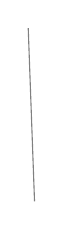
\begin{tikzpicture}\draw[gray] (0,0)--(-.08,2.2);\end{tikzpicture}}}

Nous admettrons que ces relations restent valables dans le cas de la cohomologie cristalline. Alors l'homomorphisme (8.2.1) s'interprète comme l'homomorphisme
\[
(8.3.2)\qquad u''_2:\operatorname{Tors}^{n-1}(X)\otimes_W k\longrightarrow\operatorname{Tors}^{n+1}(X)\otimes_W k
\]
induit par l'homomorphisme $H^{n-1}(X)\to H^{n+1}(X)$, cup-produit par la classe de polarisation de $X\subset P_k^r$. La chose importante pour nous est que ce morphisme (donc son Ker) ne dépend plus du choix de $Y$, donc \deleted{aussi du}\deleted{\unsure{il en est de même}}\inserted{le} dernier terme de (8.1.3) \deleted{ne dépend} (qui est le dual de ce Ker) ne dépend plus de $Y$. Un autre point important est que, $E(Y)$ étant sans torsion, il a même rang que $E(Y)\otimes_W k$ intervenant dans (8.1.3) (et en particulier, si on a un endomorphisme de $E(Y)$, par exemple un frobenius, les valeurs propres de l'endomorphisme induit de $E(Y)\otimes k$ sont bien les réductions

\mspage{3}
